\documentclass{article}
\usepackage{graphicx}

\begin{document}

\title{Project Report: Random Number Generator}
\author{Sudarshan Shivashankar}
\date{\today}

\maketitle

\section{Introduction}
The Random Number Generator (RNG) is a circuit that generates random numbers using electronic components. In this project, we will design and implement an RNG using a breadboard, a Seven-Segment Display, a 7474 Flip-Flop, a 7447 Decoder, a 7684 Clock, a 555 IC, resistors (1k$\Omega$, 1M$\Omega$), capacitors (100nF, 10nF), and jump wires. This report provides a detailed description of the components used, the circuit design, a block diagram of the system, and an output image.

\section{Components}
The following components are required for this project:
\begin{enumerate}
  \item Breadboard: Provides a platform for connecting and prototyping electronic circuits.
  \item Seven-Segment Display: Displays the generated random number in decimal format.
  \item 7474 Flip-Flop: A dual positive-edge-triggered D-type flip-flop used for storing and controlling the random number generation.
  \item 7447 Decoder: Converts the binary output from the flip-flop to the appropriate signals for the Seven-Segment Display.
  \item 7684 Clock: Generates clock pulses to trigger the flip-flop.
  \item 555 IC: An integrated circuit used as an astable multivibrator to generate clock pulses.
  \item Resistors: A 1k$\Omega$ resistor and a 1M$\Omega$ resistor are used to set the timing and voltage levels in the circuit.
  \item Capacitors: A 100nF capacitor and a 10nF capacitor are used for timing and stability purposes.
  \item Jump Wires: Used to establish connections between the components on the breadboard.
\end{enumerate}

\section{Description of the Circuit}
The circuit consists of the following key components:
\begin{enumerate}
  \item 555 IC: Configured as an astable multivibrator to generate clock pulses. The timing is determined by the values of the resistors and capacitors connected to the IC.
  \item 7684 Clock: Receives the clock pulses from the 555 IC and provides them to the flip-flop.
  \item 7474 Flip-Flop: Connected to the clock, it stores and controls the random number generation process.
  \item 7447 Decoder: Takes the binary output from the flip-flop and converts it to the appropriate signals for the Seven-Segment Display.
  \item Seven-Segment Display: Displays the generated random number in decimal format.
\end{enumerate}

The circuit is designed as follows:
\begin{enumerate}
  \item Connect the power supply to the breadboard.
  \item Place the 555 IC on the breadboard and connect the resistors and capacitors to the appropriate pins to configure it as an astable multivibrator.
  \item Connect the clock output of the 555 IC to the clock input of the 7684 Clock.
  \item Connect the power and ground pins of the flip-flop and decoder to the power supply and ground respectively.
  \item Connect the clock output of the 7684 Clock to the clock input of the flip-flop.
  \item Connect the binary outputs of the flip-flop to the inputs of the decoder.
  \item Connect the output pins of the decoder to the appropriate input pins of the Seven-Segment Display.
  \item Connect the power and ground pins of the Seven-Segment Display to the power supply and ground respectively.
\end{enumerate}
\section{Working of the Circuit}
Description of the Random Number Generator Circuit using Shift Registers:
\begin{itemize}
\item The random number generator circuit is designed to generate random numbers using shift registers, providing a versatile and reliable solution for applications that require randomness. The circuit incorporates various components, including a breadboard, seven-segment display, decoder, flip-flops, XOR gate, 555 timer IC, resistors, capacitors, and jumper wires.


\item At the core of the circuit is the shift register, constructed using two D flip-flops (7474 ICs) and an XOR gate (7486 IC). The shift register operates based on the clock signal generated by the 555 timer IC. The clock signal serves as the synchronization mechanism, ensuring the precise shifting of data within the shift register.


\item The clock signal generated by the 555 timer circuit is connected to the CLOCK input of the D flip-flops, enabling the sequential shifting of data through the flip-flops. This shifting action creates a cascading effect, allowing the circuit to generate a sequence of random bits.


\item The output of each D flip-flop is connected to the Decoder IC (7447 IC), which converts the binary input into a corresponding output that can be displayed on the seven-segment display. The connections between the flip-flops and the decoder are carefully established to ensure the proper mapping of binary values to the display segments.


\item The seven-segment display, a common anode type, is connected to the Decoder IC (7447 IC) following the prescribed pin connections. This display arrangement allows the generated random numbers to be visually represented in a human-readable format.


\item Power and ground connections are established for all components to ensure proper operation and signal integrity. The circuit requires a stable power supply, and the voltage specifications of each component should be respected to prevent damage and ensure accurate performance.


\item The random number generator circuit offers various applications, such as simulations, gaming, cryptography, testing, art, research, and decision-making. By following the circuit diagram and carefully assembling the components, users can create a functional and reliable random number generator capable of providing high-quality random numbers for their specific needs.
\end{itemize}\\
\\
\section{Output Image}
\begin{figure}[h]
  \centering
  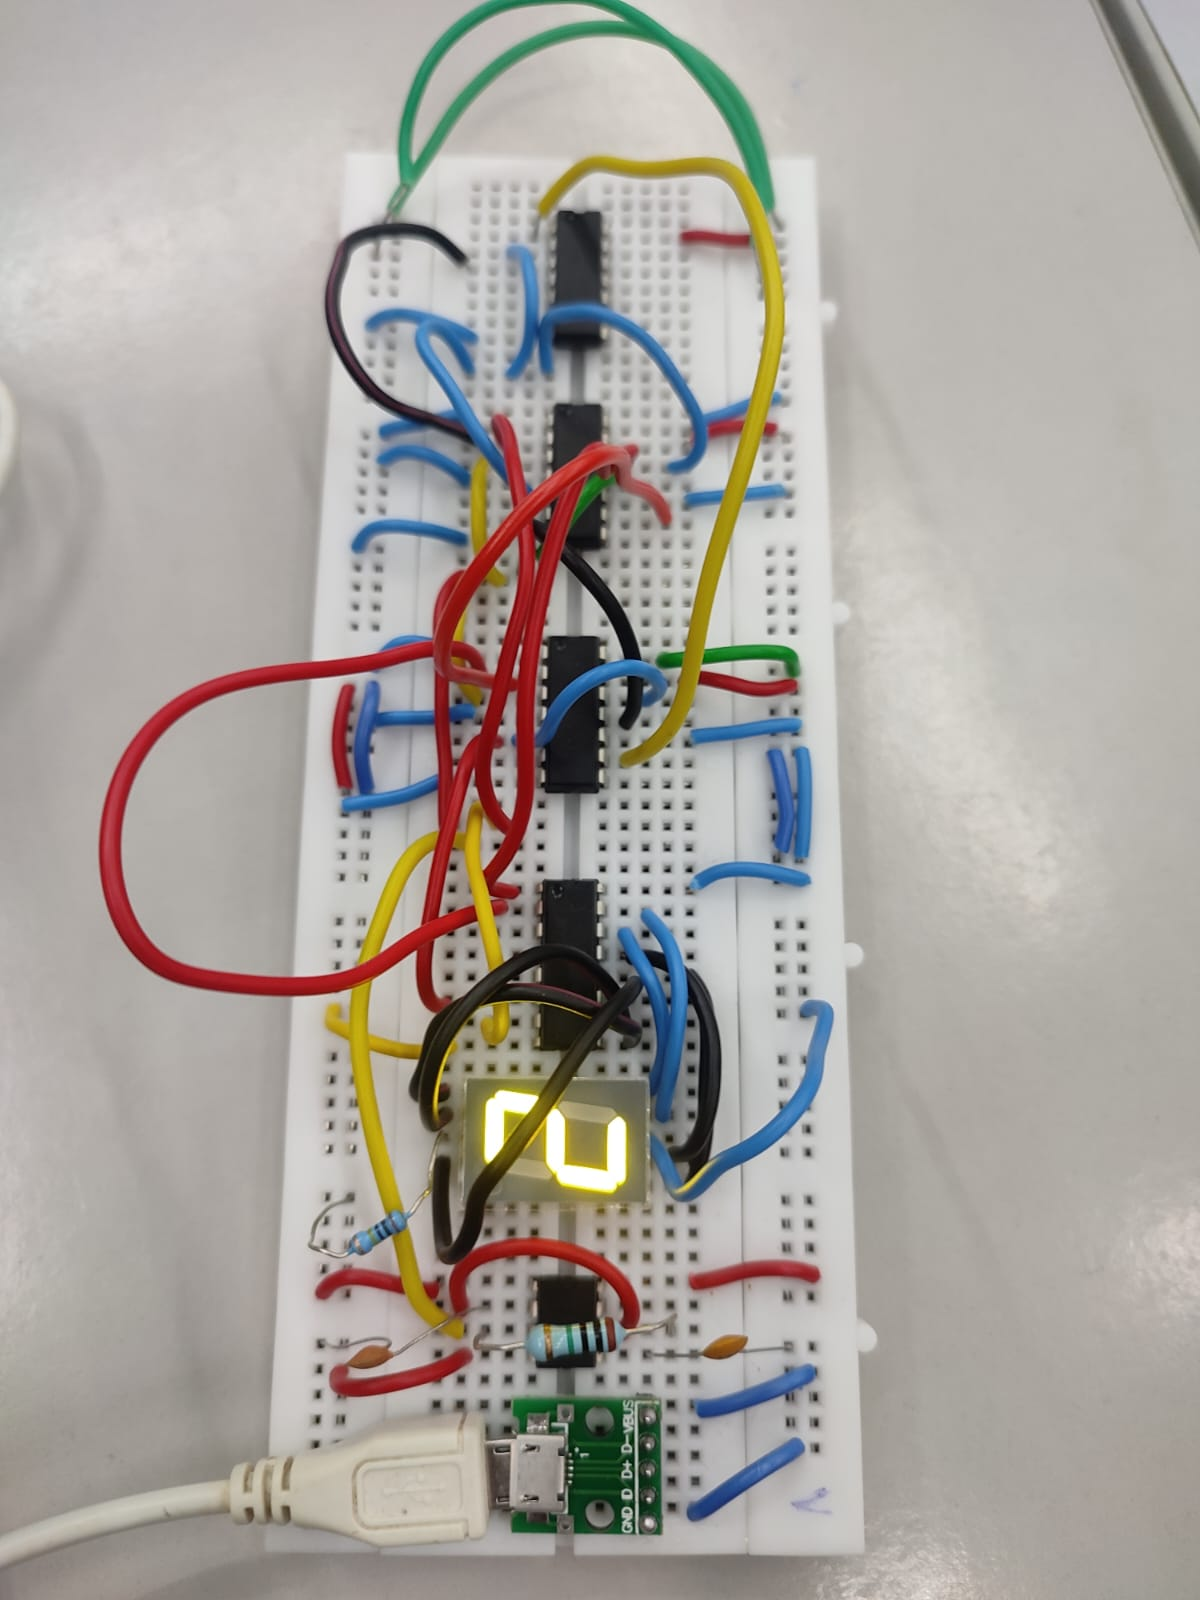
\includegraphics[width=0.8\textwidth]{/home/sudarshan/Downloads/prv2.jpeg}
  \caption{Completed circuit with the Seven-Segment Display displaying a random number.}
\end{figure}
\begin{figure}[h]
  \centering
  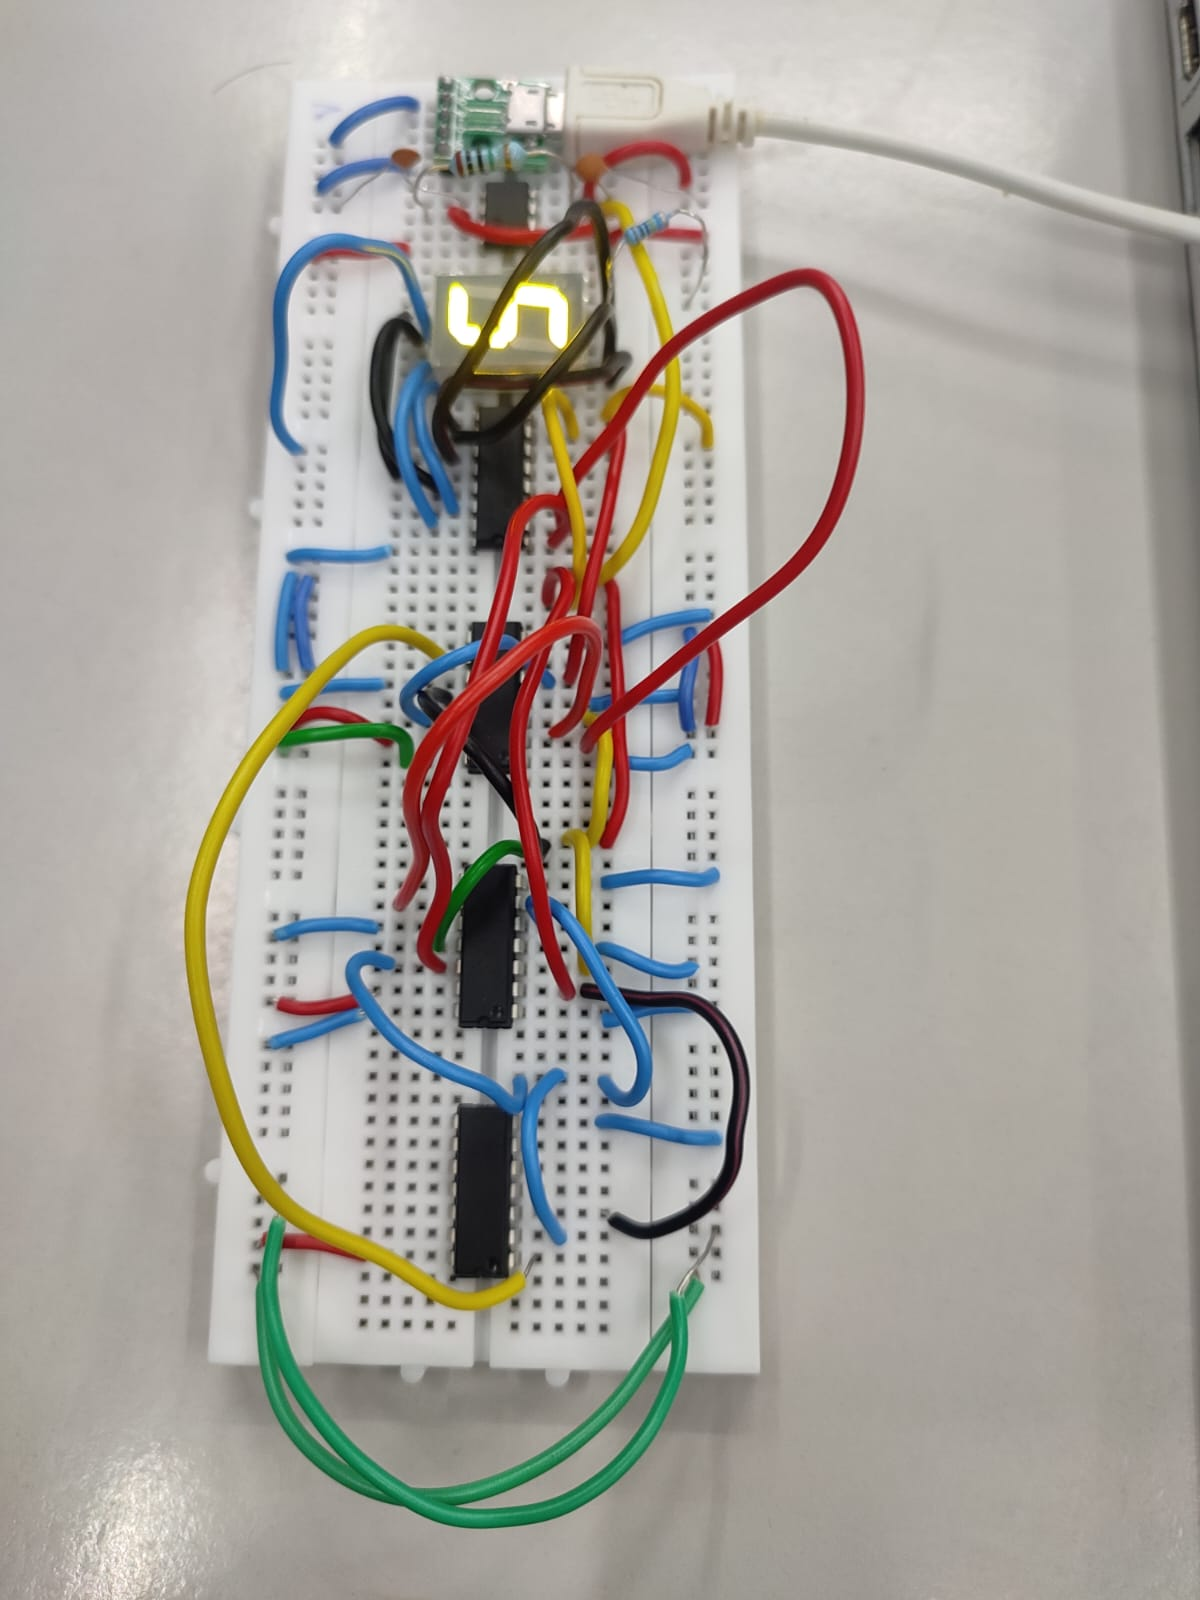
\includegraphics[width=0.8\textwidth]{/home/sudarshan/Downloads/prvim2.jpeg}
  \caption{Completed circuit with the Seven-Segment Display displaying a random number.}
\end{figure}


%\section{Block Diagram}
\begin{figure}[h]
  \centering
  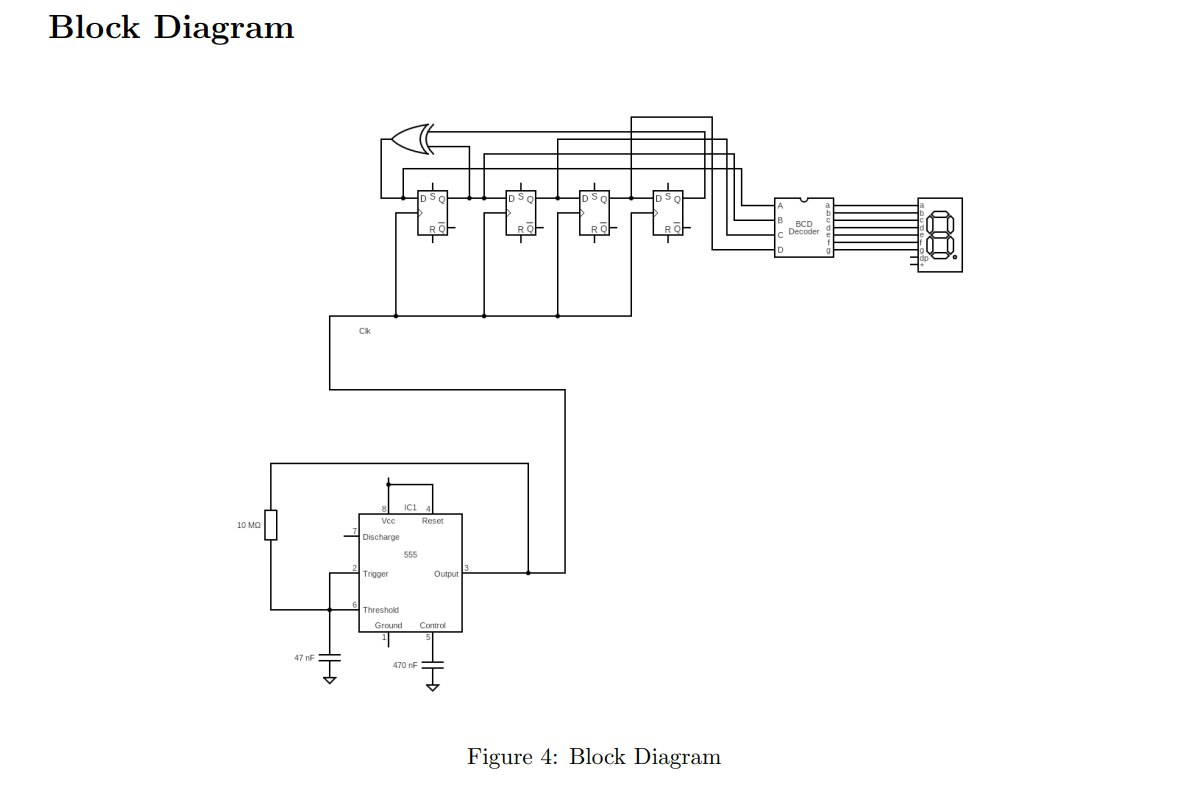
\includegraphics[width=1.5\textwidth]{/home/sudarshan/Downloads/prvimg2.jpg}
  \caption{Block diagram of the Random Number Generator circuit.}
\end{figure}

\end{document}